\graphicspath{{images/mechanics}}

\section{Mechanik}

In der Nächsten Sektion wird die Mechanik der Fotobox beschrieben.
Die Mechanik ist ein sehr wichtiger Teil der Fotobox, da sie das erste
ist, was der Endbenutzer sieht. Sie sollte daher ansprechend und so stabil
aufgebaut sein, dass sie auch bei häufigem Transport nicht beschädigt wird.
Daher werde ich nun erläutern, warum ich mich für das aktuelle Design entschieden habe
und welche Probleme ich dabei hatte.

\subsection{Design}

Da das Design der Fotobox sehr wichtig ist, habe ich verschiedene Designs ausprobiert.
Der Weg, welcher zum schlussendlichen Design geführt hat, wird in Folgendem Unterkapitel beschrieben.

\begin{figure}[H]
    \centering
    \includegraphics[width=1\textwidth]{fotobox_frontplatte_v1.png}
    \caption{Die erste Version der Frontplatte.}
    \label{fig:frontplatte_v1}
\end{figure}

In der \autoref{fig:frontplatte_v1} ist die erste Version der Frontplatte zu sehen.
Bei diesem Design, habe ich mich an schon am Markt erhältlichen Fotoboxen orientiert.
In den löchern eins und zwei sollten jeweils ein Blitz und eine LED Lampe platziert werden,
in dem mittleren Loch mit der Nummer drei sollte die Kamera platziert werden.

Jedoch hat sich herausgestellt, dass diese Design, durch die seitliche Platzierung des Blitzes
das Bild nicht einheitlich ausleuchtet, und einen seitlichen Schatten hinter dem 
Motiv wirft. Was die Qualität der Bilder, wie in \autoref{fig:seitlicher_blitzt}
zu sehen ist, deutlich verringert, da das Bild auch nicht einheitlich ausgeleuchtet wird.

\newpage
\begin{figure}[H]
    \centering
    \includegraphics[width=0.8\textwidth]{blitz_seitlich.JPG}
    \caption{Beispielbild mit seitlichem Blitz.}
    \label{fig:seitlicher_blitzt}
\end{figure}

In der \autoref{fig:seitlicher_blitzt} ist zu sehen, dass durch die seitliche Platzierung des Blitzes 
auf der linken Seite neben dem Motiv ein Schatten entsteht. Dieser Schatten ist unerwünscht und sollte
durch ein zentrales Blitzlicht vermieden werden.

\begin{figure}[H]
    \centering
    \includegraphics[width=0.8\textwidth]{blitz_vorne.JPG}
    \caption{Beispielbild mit zentralem Blitz.}
    \label{fig:zentraler_blitz}
\end{figure}

In der \autoref{fig:zentraler_blitz} ist zu sehen, dass durch die zentrale Platzierung des Blitzes,
das Bild deutlich besser ausgeleuchtet ist und keine seitlichen Schatten entstehen.
Darum habe ich mich dazu entschieden, das Design noch einmal zu überarbeiten und
den Blitzt zentral über der Kamera zu platzieren.

\newpage

Hier in \autoref{fig:frontplatte_v2} ist das überarbeitete Design zu sehen.
Im Gegensatz zur ersten Version, ist das neue Design 
nun höher, wie breit, wodurch es möglich ist, den Blitzt oberhalb der Kamera in 
Öffnung eins zu platzieren. In den Öffnungen zwei und drei sind die LED Lampen,
durch die auch bei der Vorschau, obwohl die Lichtquellen neben der Kamera sind,
eine symmetrische Beleuchtung des Motivs gewährleistet ist.

\begin{figure}[H]
    \centering
    \includegraphics[width=0.75\textwidth]{fotobox_frontplatte_v2.png}
    \caption{Die erste Version der Frontplatte.}
    \label{fig:frontplatte_v2}
\end{figure}

Dieses Design bringt zudem weitere Vorteile mit sich. Besonders hervorzuheben
ist die Tatsache, dass die Form der Fotobox einem menschlichen Gesicht ähnelt.
Dies hat einen positiven psychologischen Effekt auf die Nutzerinnen und Nutzer:
Menschen fühlen sich in der Regel wohler und entspannter, wenn sie das Gefühl
haben, jemandem ins Gesicht zu blicken, anstatt lediglich vor einer anonymen,
leblosen Holzbox zu stehen. Die vertraute, „menschliche“ Gestaltung kann
Hemmschwellen abbauen und dazu beitragen, dass sich die Personen natürlicher und
ungezwungener vor der Kamera verhalten. Dadurch entstehen oft authentischere und
ausdrucksstärkere Fotos, was den Gesamteindruck und die Nutzererfahrung der Fotobox
deutlich verbessert.

\newpage

\subsection{Zusammenbau}

Im folgenden Kapitel wird der Zusammenbau der Fotobox beschrieben.
Da die Fotobox aus mehreren Teilen besteht, welche alle zuerst Zugeschnitten,
und alle nötigen Öffnungen gebohrt und gefräst werden müssen.

\subsubsection{Rohmaterial}

Das Rohmaterial, für welches ich mich entschieden habe, ist 18 mm dickes buchen
Leimholz, wie in \autoref{fig:rohmaterial} zu sehen ist.

\begin{figure}[H]
    \centering
    \includegraphics[width=0.75\textwidth]{rohmaterial.JPG}
    \caption{Das Rohmaterial der Fotobox.}
    \label{fig:rohmaterial}
\end{figure}

Ich habe mich für Leimholz aus Buche entschieden, da es durch die Verleimung der
einzelnen Holzlamellen eine hohe Formstabilität aufweist und sich kaum verzieht.
Zudem ist Buche ein sehr hartes Holz, wodurch die Box sehr stabil ist.
Jedoch ist Buche durch diese Eigenschaften auch schwerer zu verarbeiten,
als ein weicheres Holt und durch das höhere Gewicht, wird die Box auch schwerer.

\newpage

\subsubsection{Zuschnitt}

Zuerst sollten aus den beiden Platten mit den Maßen 2000 mm x 300 mm x 18 mm und 
2000 mm x 500 mm x 18 mm die einzelnen Teile der Fotobox auf der Kreissäge
zugeschnitten werden. In der Abbildung \autoref{fig:zuschnitt_mit_kreissaege} ist der grobe 
Zuschnitt der Platten auf der Kreissäge zu sehen.

\begin{figure}[H]
    \centering
    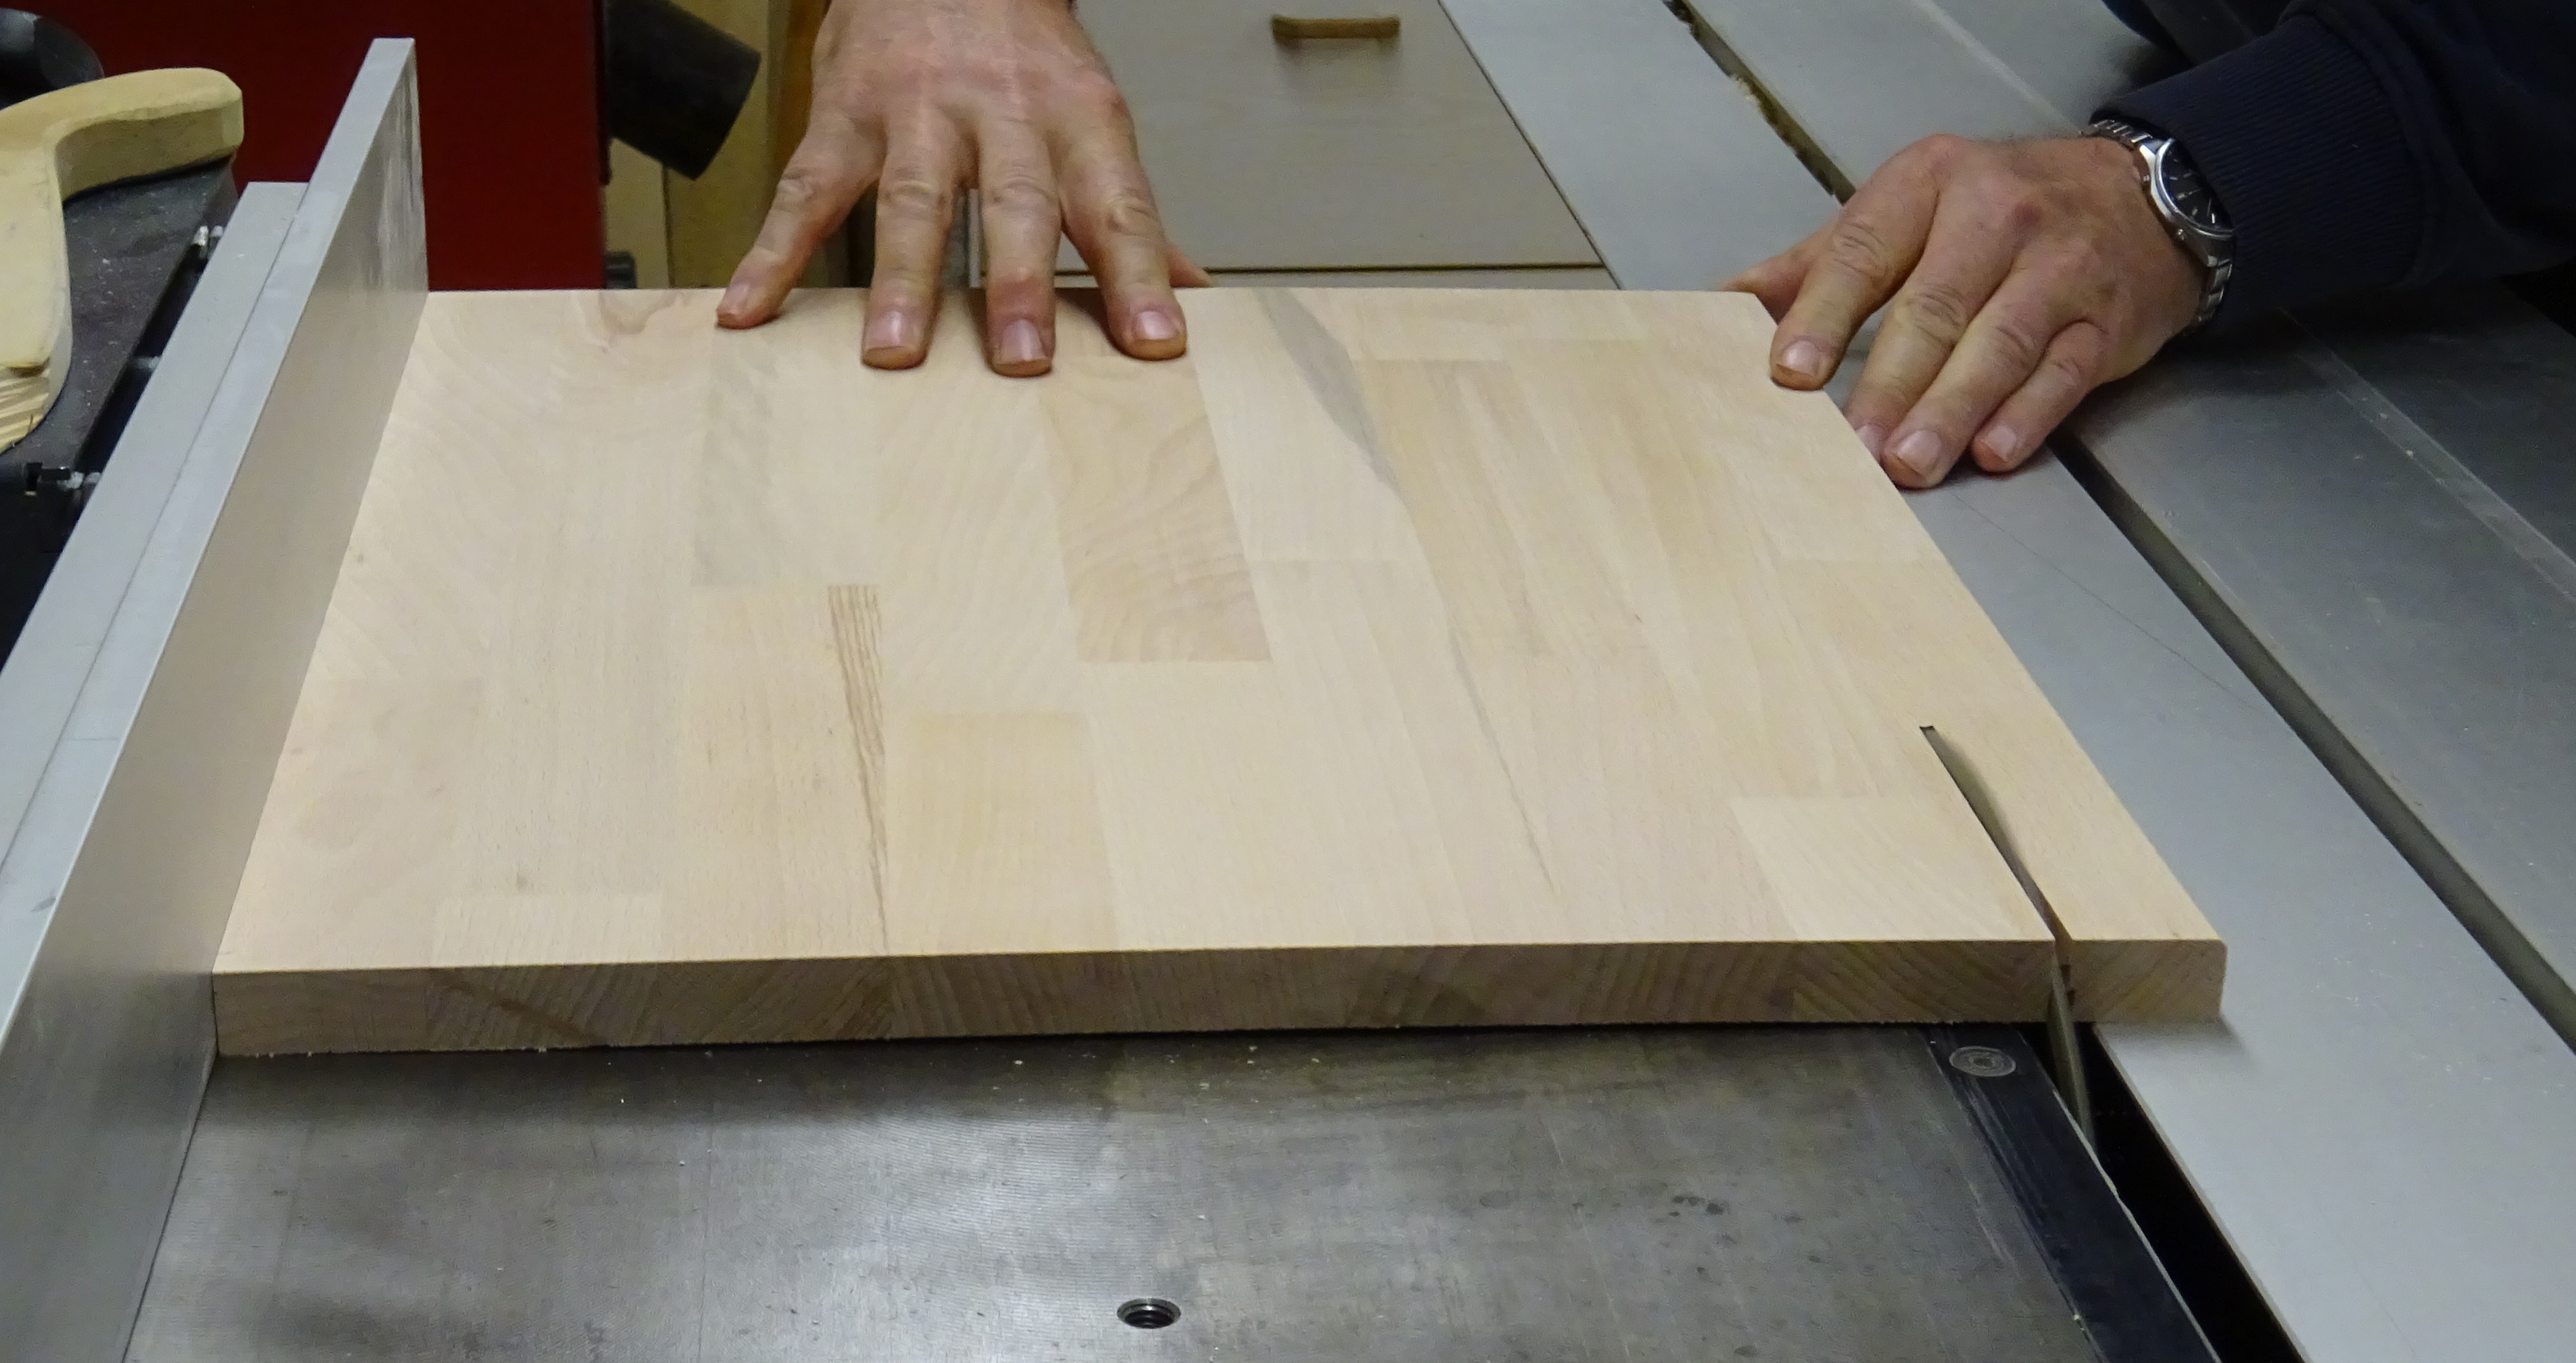
\includegraphics[width=0.75\textwidth]{zuschnitt_mit_kreissaege.JPG}
    \caption{Der Zuschnitt der Platten auf der Kreissäge.}
    \label{fig:zuschnitt_mit_kreissaege}
\end{figure}

Nach dem ersten groben Zuschnitt, wurde das Kreissägeblatt auf 45° gestellt, um
die kanten der Platten mit einer Fase zu versehen. Durch diese Fase, können die Platten
wie in \autoref{fig:fotobox_kanten} zu sehen ist, besser zusammengefügt werden.

\begin{figure}[H]
    \centering
    \includegraphics[width=0.5\textwidth]{fotobox_kanten.png}
    \caption{Zusammenfügen der Platten.}
    \label{fig:fotobox_kanten}
\end{figure}

Was erstens die Stabilität der Box erhöht und zweitens die Optik verbessert. 
Außerdem, wurde bei diesem Zweiten zuschnitt, auch darauf geachtet, dass die
Platten genau aneinander passen, da beim ersten Zuschnitt nur grobe Maße
genommen wurden.

\newpage

Nach dem alle Platten auf die richtige Größe zugeschnitten wurden und durch
Zusammensetzen, wie in \autoref{fig:fotobox_zusamensetzen_test}, der Box überprüft
wurde, dass die Platten auch ohne Lücken aneinander passen, wurden die Öffnungen
für die Kamera, den Blitz und die LED Lampen gefräst und gebohrt.

\begin{figure}[H]
    \centering
    \includegraphics[width=0.6\textwidth]{fotobox_zusamensetzen_test.JPG}
    \caption{Überprüfen der Platten auf Passgenauigkeit der Platten.}
    \label{fig:fotobox_zusamensetzen_test}
\end{figure}

Um die Runden Öffnungen für die Kamera, die LED Lampen zu bohren, wurde die Frontplatte
auf der Standbohrmaschine eingespannt, und wie in \autoref{fig:fotobox_loch_saegen} zu sehen ist,
wurde mit einer Lochsäge die Öffnung für die Kamera und die LED Lampen gebohrt.

\begin{figure}[H]
    \centering
    \includegraphics[width=0.75\textwidth]{fotobox_loch_saegen.JPG}
    \caption{Die Standbohrmaschine mit der Lochsäge.}
    \label{fig:fotobox_loch_saegen}
\end{figure}

Um die Öffnungen für den Blitz und Laptop auszuschneiden, wurde die Fräse verwendet.
Dazu wurde die Frontplatte auf der Fräse eingespannt und wie in
\autoref{fig:fotobox_fraesen} zu sehen ist, wurden die rechteckigen Öffnungen
für den Blitz und den Laptop gefräst. Außerdem wurde bei der Öffnung für den Blitz
noch eine Vertiefung gefräst, in welche ein milchiges Acrylglas eingesetzt werden kann.

\begin{figure}[H]
    \centering
    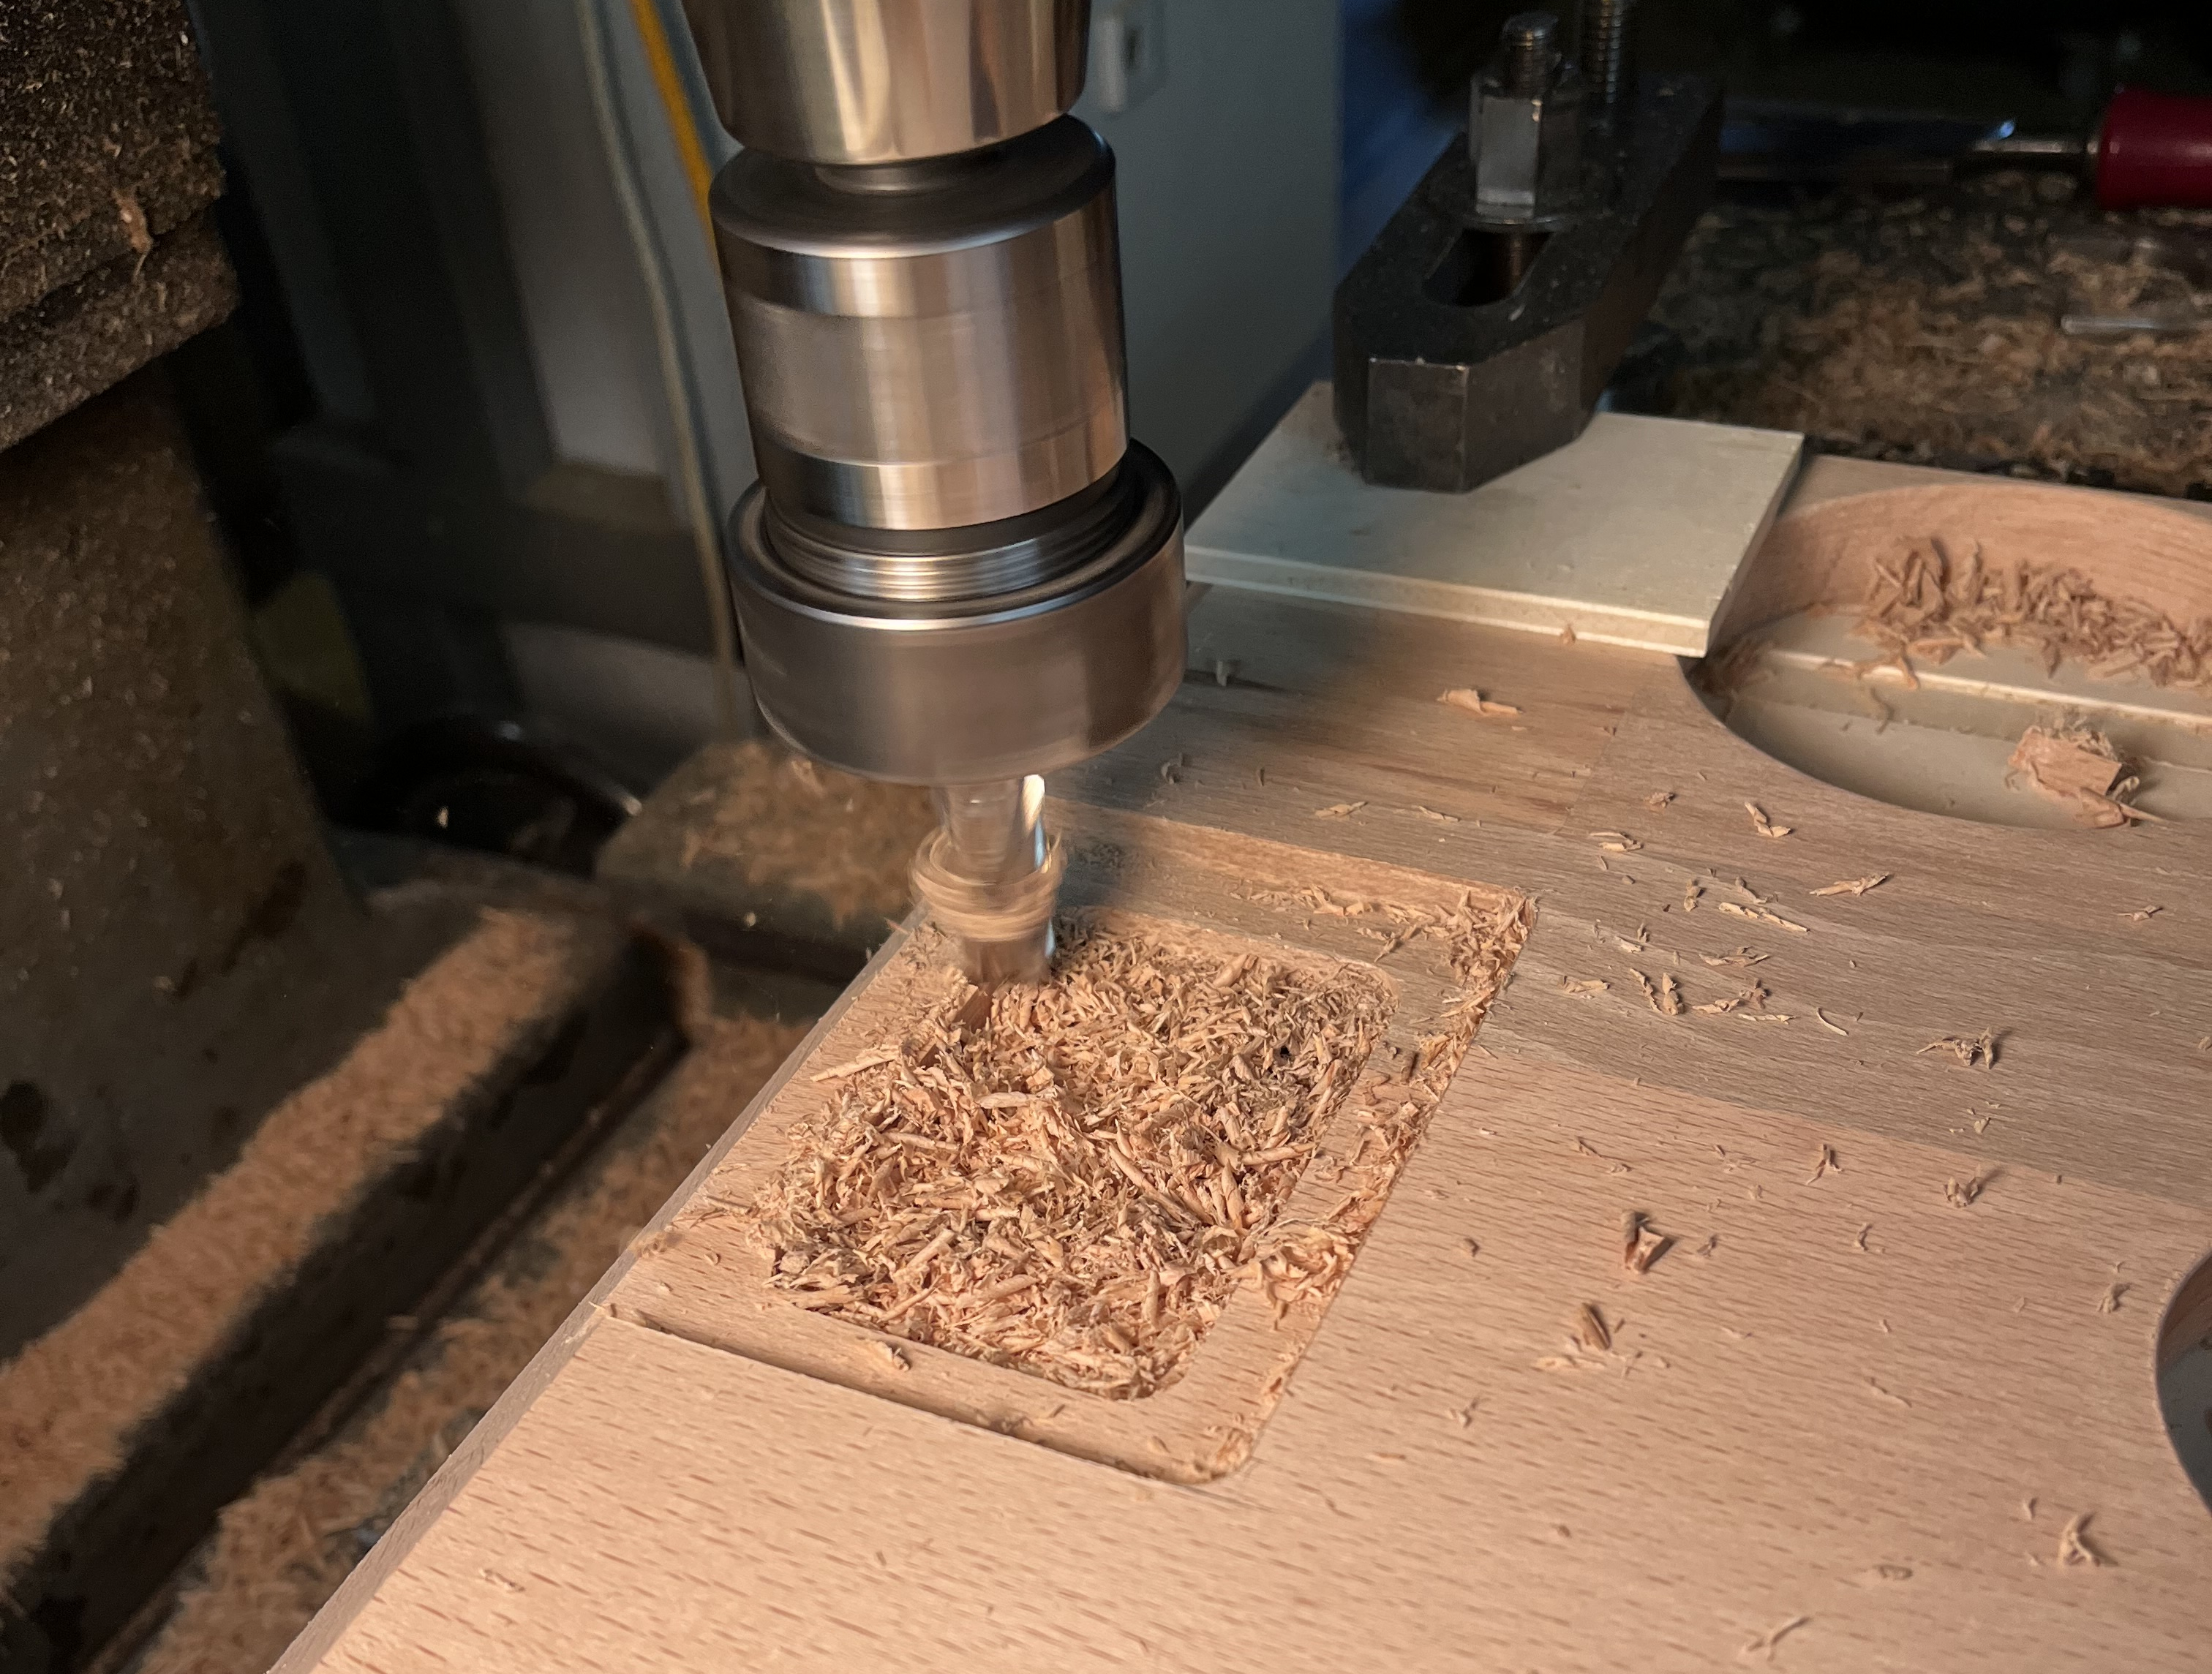
\includegraphics[width=0.75\textwidth]{fotobox_fraesen.JPG}
    \caption{Fräsen der Öffnungen für den Blitz und Laptop.}
    \label{fig:fotobox_fraesen}
\end{figure}

\newpage

\subsubsection{Zusammenleimen der Box}

Bevor die Box zusammengeleimt wird, wurde überprüft, ob auch alle Öffnungen 
vorhanden sind, dazu wurden alle Teile wie in \autoref{fig:fotobox_fertige_teile}
aufgelegt. 

\begin{figure}[H]
    \centering
    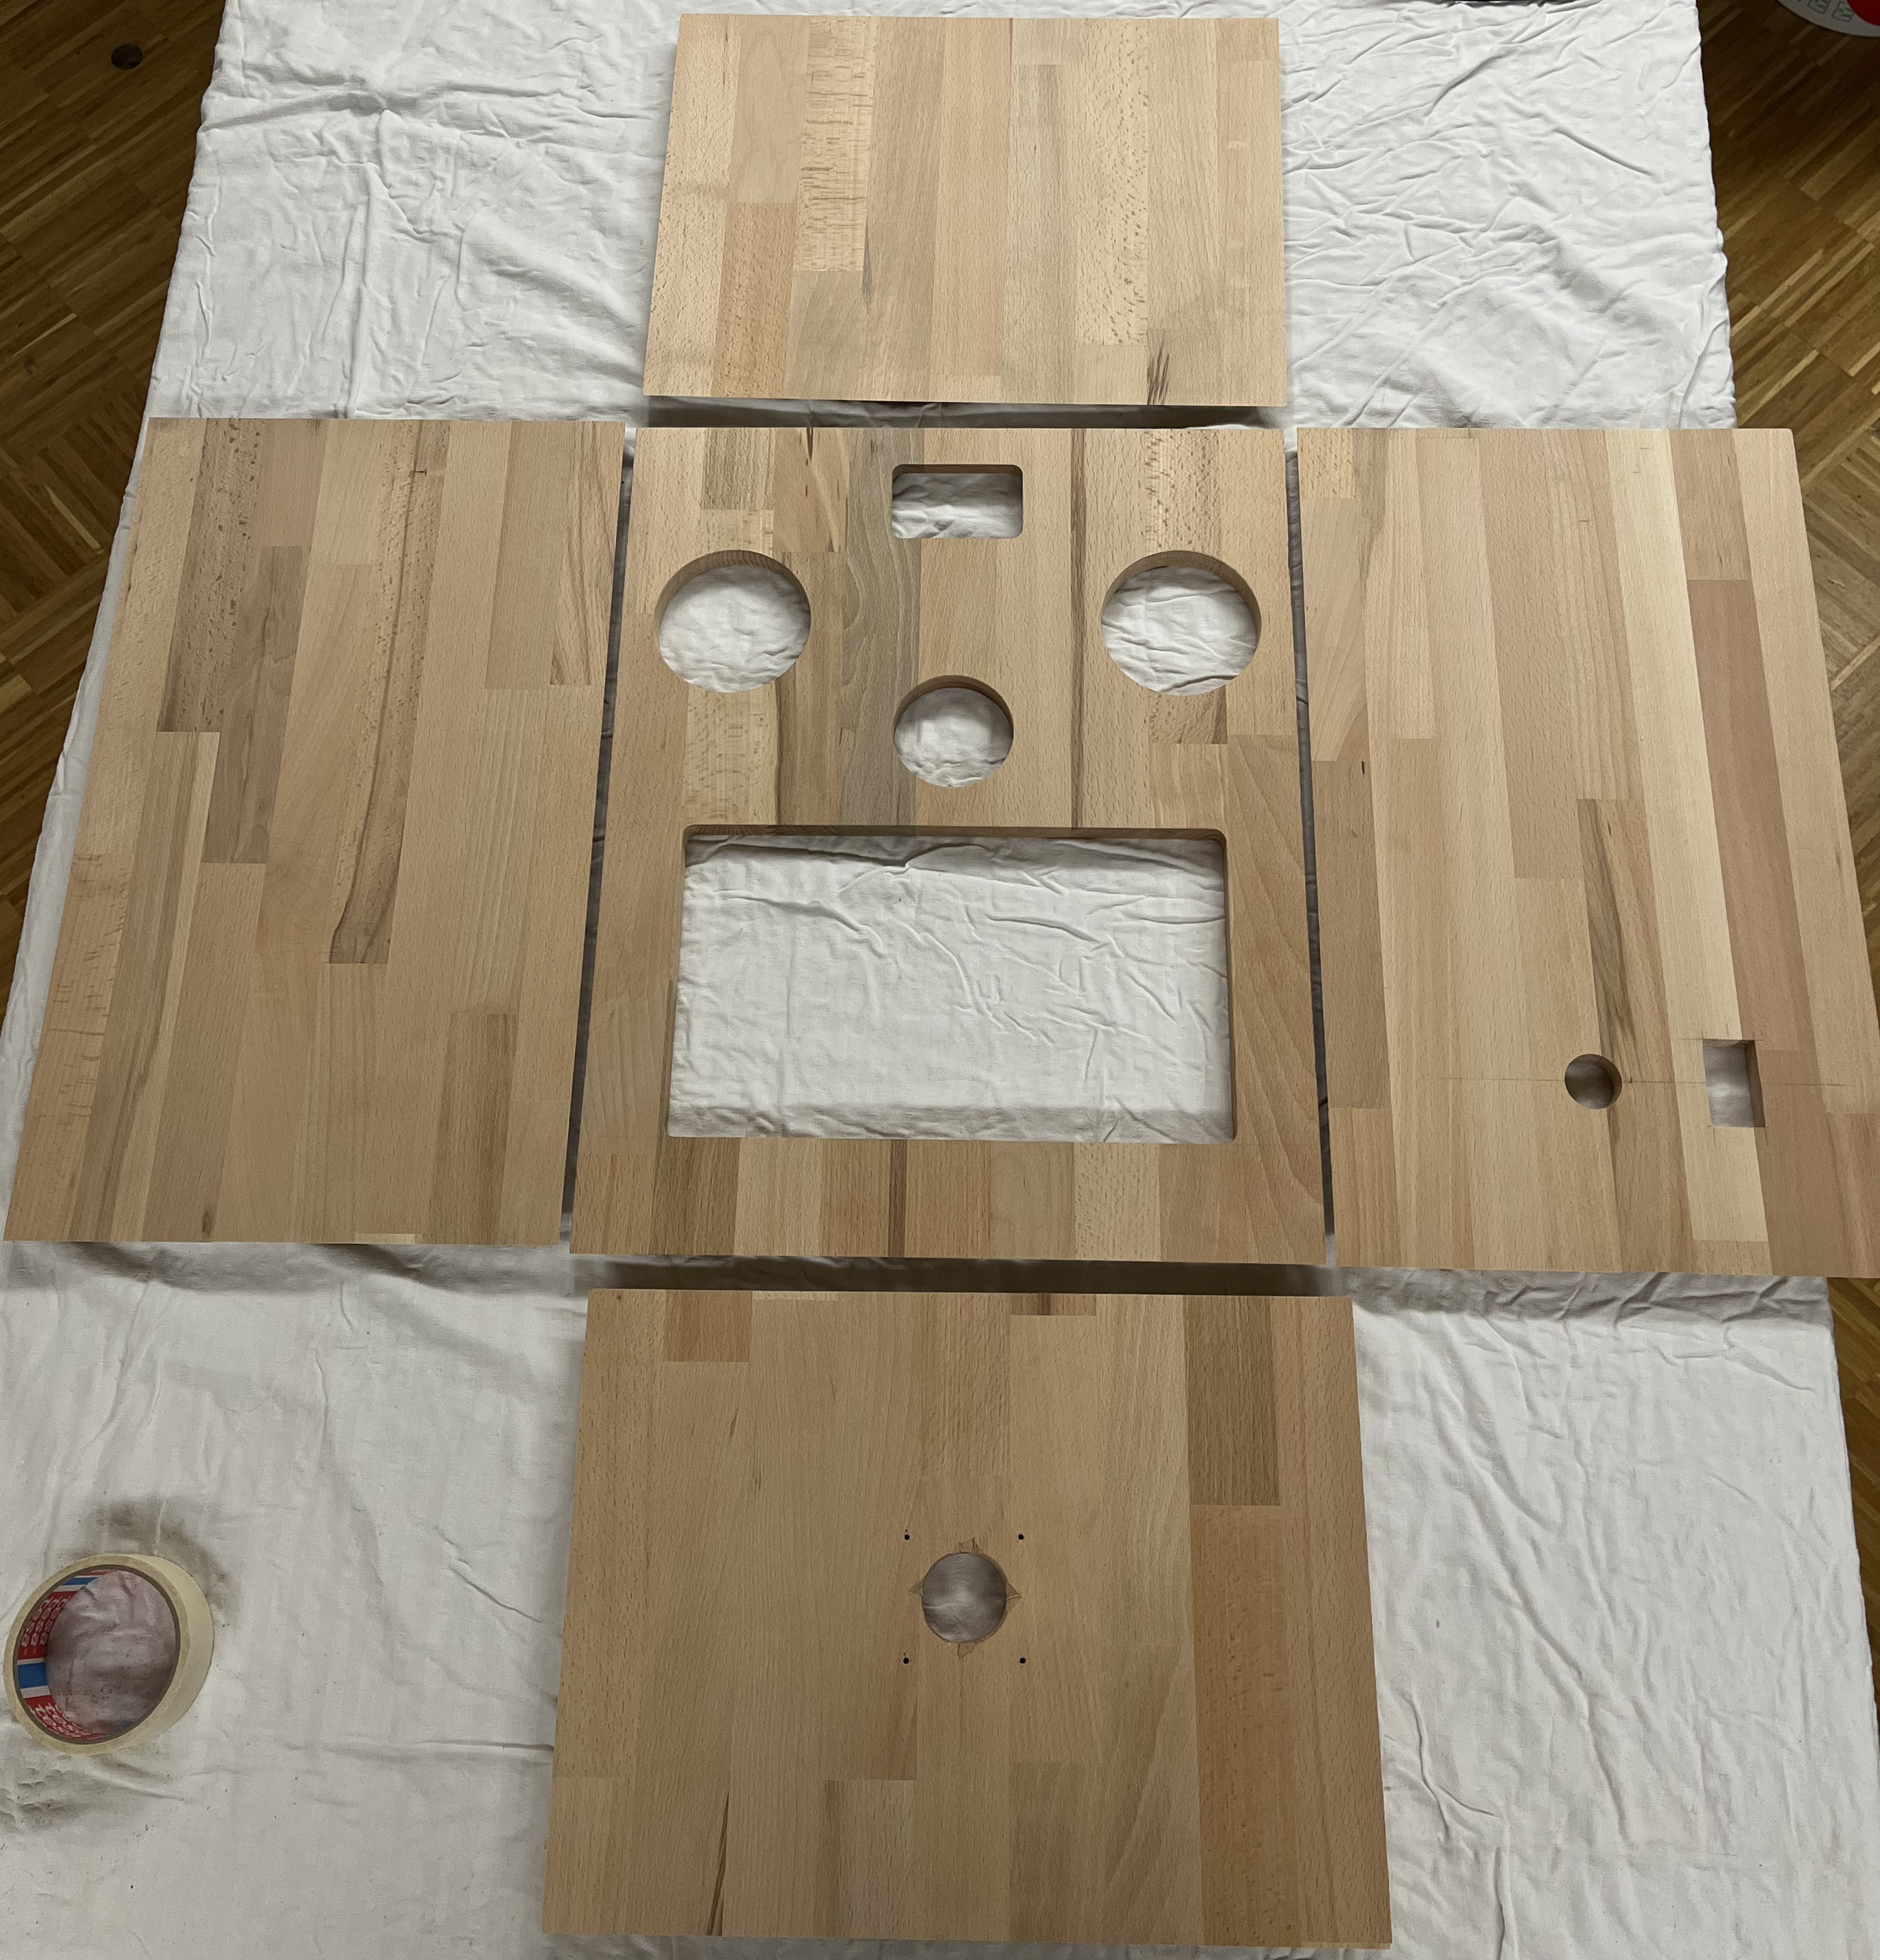
\includegraphics[width=0.75\textwidth]{fotobox_fertige_teile.JPG}
    \caption{Auflegen der Fertigen Teile.}
    \label{fig:fotobox_fertige_teile}
\end{figure}

Anschließend wurde auf alle Kanten der Platten Holzleim aufgetragen, wie in 
\autoref{fig:fotobox_verleimen} und die Platten wurden zusammengeleimt.

\begin{figure}[H]
    \centering
    \includegraphics[width=0.75\textwidth]{fotobox_verleimen.JPG}
    \caption{Auftragen des Holzleims.}
    \label{fig:fotobox_verleimen}
\end{figure}

\newpage

Nachdem der Leim der Platten getrocknet ist, wurde das Kreppband entfernt und
alle herausquellenden Leimreste wurden entfernt. Anschließend wurden auf 
dem Frästisch alle von Vorne sichtbaren Kanten mit einem Kantenfräser mit einem
Radius von 8mm abgerundet. Dieser Arbeitsschritt ist in \autoref{fig:fotobox_fraesen}

\begin{figure}[H]
    \centering
    \includegraphics[width=0.75\textwidth]{kanten_fraesen.JPG}
    \caption{Fräsen der Kanten.}
    \label{fig:fotobox_fraesen}
\end{figure}

\newpage

\subsubsection{Bauen der Halterungen}

Als Nächstes wurden die Halterungen für die Kamera, den Blitz und den Laptop gebaut.


Für die Halterung des Blitzes, mussten in ein Flacheisen, zwei m6 Gewinde
eingeschnitten werden, um anschließend, dies ist in \autoref{fig:fertiges_gewinde}
zu sehen ist eine Gewindestange einzuschrauben.

\begin{figure}[H]
    \centering
    \includegraphics[width=0.75\textwidth]{fertiges_gewinde.JPG}
    \caption{Flacheisen mit Gewinde.}
    \label{fig:fertiges_gewinde}
\end{figure}

Um ein Gewinde der Größe M6 herzustellen, muss zuvor ein Kernloch mit einem
Durchmesser von 5mm gebohrt werden. Der entsprechende Arbeitsschritt wird in
\autoref{fig:loch_bohren} gezeigt.

\begin{figure}[H]
    \centering
    \includegraphics[width=0.75\textwidth]{loch_bohren.JPG}
    \caption{Bohren des Lockes im Flacheisen.}
    \label{fig:loch_bohren}
\end{figure}

\newpage

Anschließend wird das gebohrte Loch mit einem Kegelsenker bearbeitet, wodurch
der beim Bohren entstandene Grat entfernt wird, sichtbar in \autoref{fig:loch_senken}.

\begin{figure}[H]
    \centering
    \includegraphics[width=0.75\textwidth]{loch_senken.JPG}
    \caption{Entgraten des Loches.}
    \label{fig:loch_senken}
\end{figure}

Als letzter Schritt wird nun das Gewinde mit einem Gewindeschneider geschnitten,
wie in Abbildung \autoref{fig:gewinde_schneiden} dargestellt.

\begin{figure}[H]
    \centering
    \includegraphics[width=0.75\textwidth]{gewinde_schneiden.JPG}
    \caption{Schneiden des Gewindes.}
    \label{fig:gewinde_schneiden}
\end{figure}

\newpage

Die fertige halterung 


\subsubsection{Schleifen und Ölen der Box}

Nachdem die Box zusammengeleimt, die Ecken abgerundet und die Halterungen
gebaut wurden, wurde die gesamte Oberfläche sorgfältig geschliffen.
Dabei kamen zunächst grobere Schleifpapiere zum Einsatz, um Unebenheiten zu
beseitigen und die Übergänge zwischen den verleimten Holzleisten zu glätten.
Anschließend wurde mit feineren Körnungen nachgearbeitet, um eine gleichmäßige,
glatte Oberfläche zu erzielen, die sich angenehm anfühlt und für die
anschließende Behandlung vorbereitet ist.

Nach dem Schleifen wurde die gesamte Box mit Leinöl behandelt.
Leinöl ist ein natürlicher Holzschutz, der das Holz vor Feuchtigkeit
und Schmutz schützt und gleichzeitig die natürliche Farbe und Maserung des Holzes
betont. Es dringt tief in das Holz ein und bildet eine schützende Schicht,
die das Holz vor äußeren Einflüssen schützt. Zudem ist Leinöl umweltfreundlich
und gesundheitlich unbedenklich, was es zu einer idealen Wahl für die
Oberflächenbehandlung von Möbeln und Holzobjekten macht.


\begin{figure}[H]
    \centering
    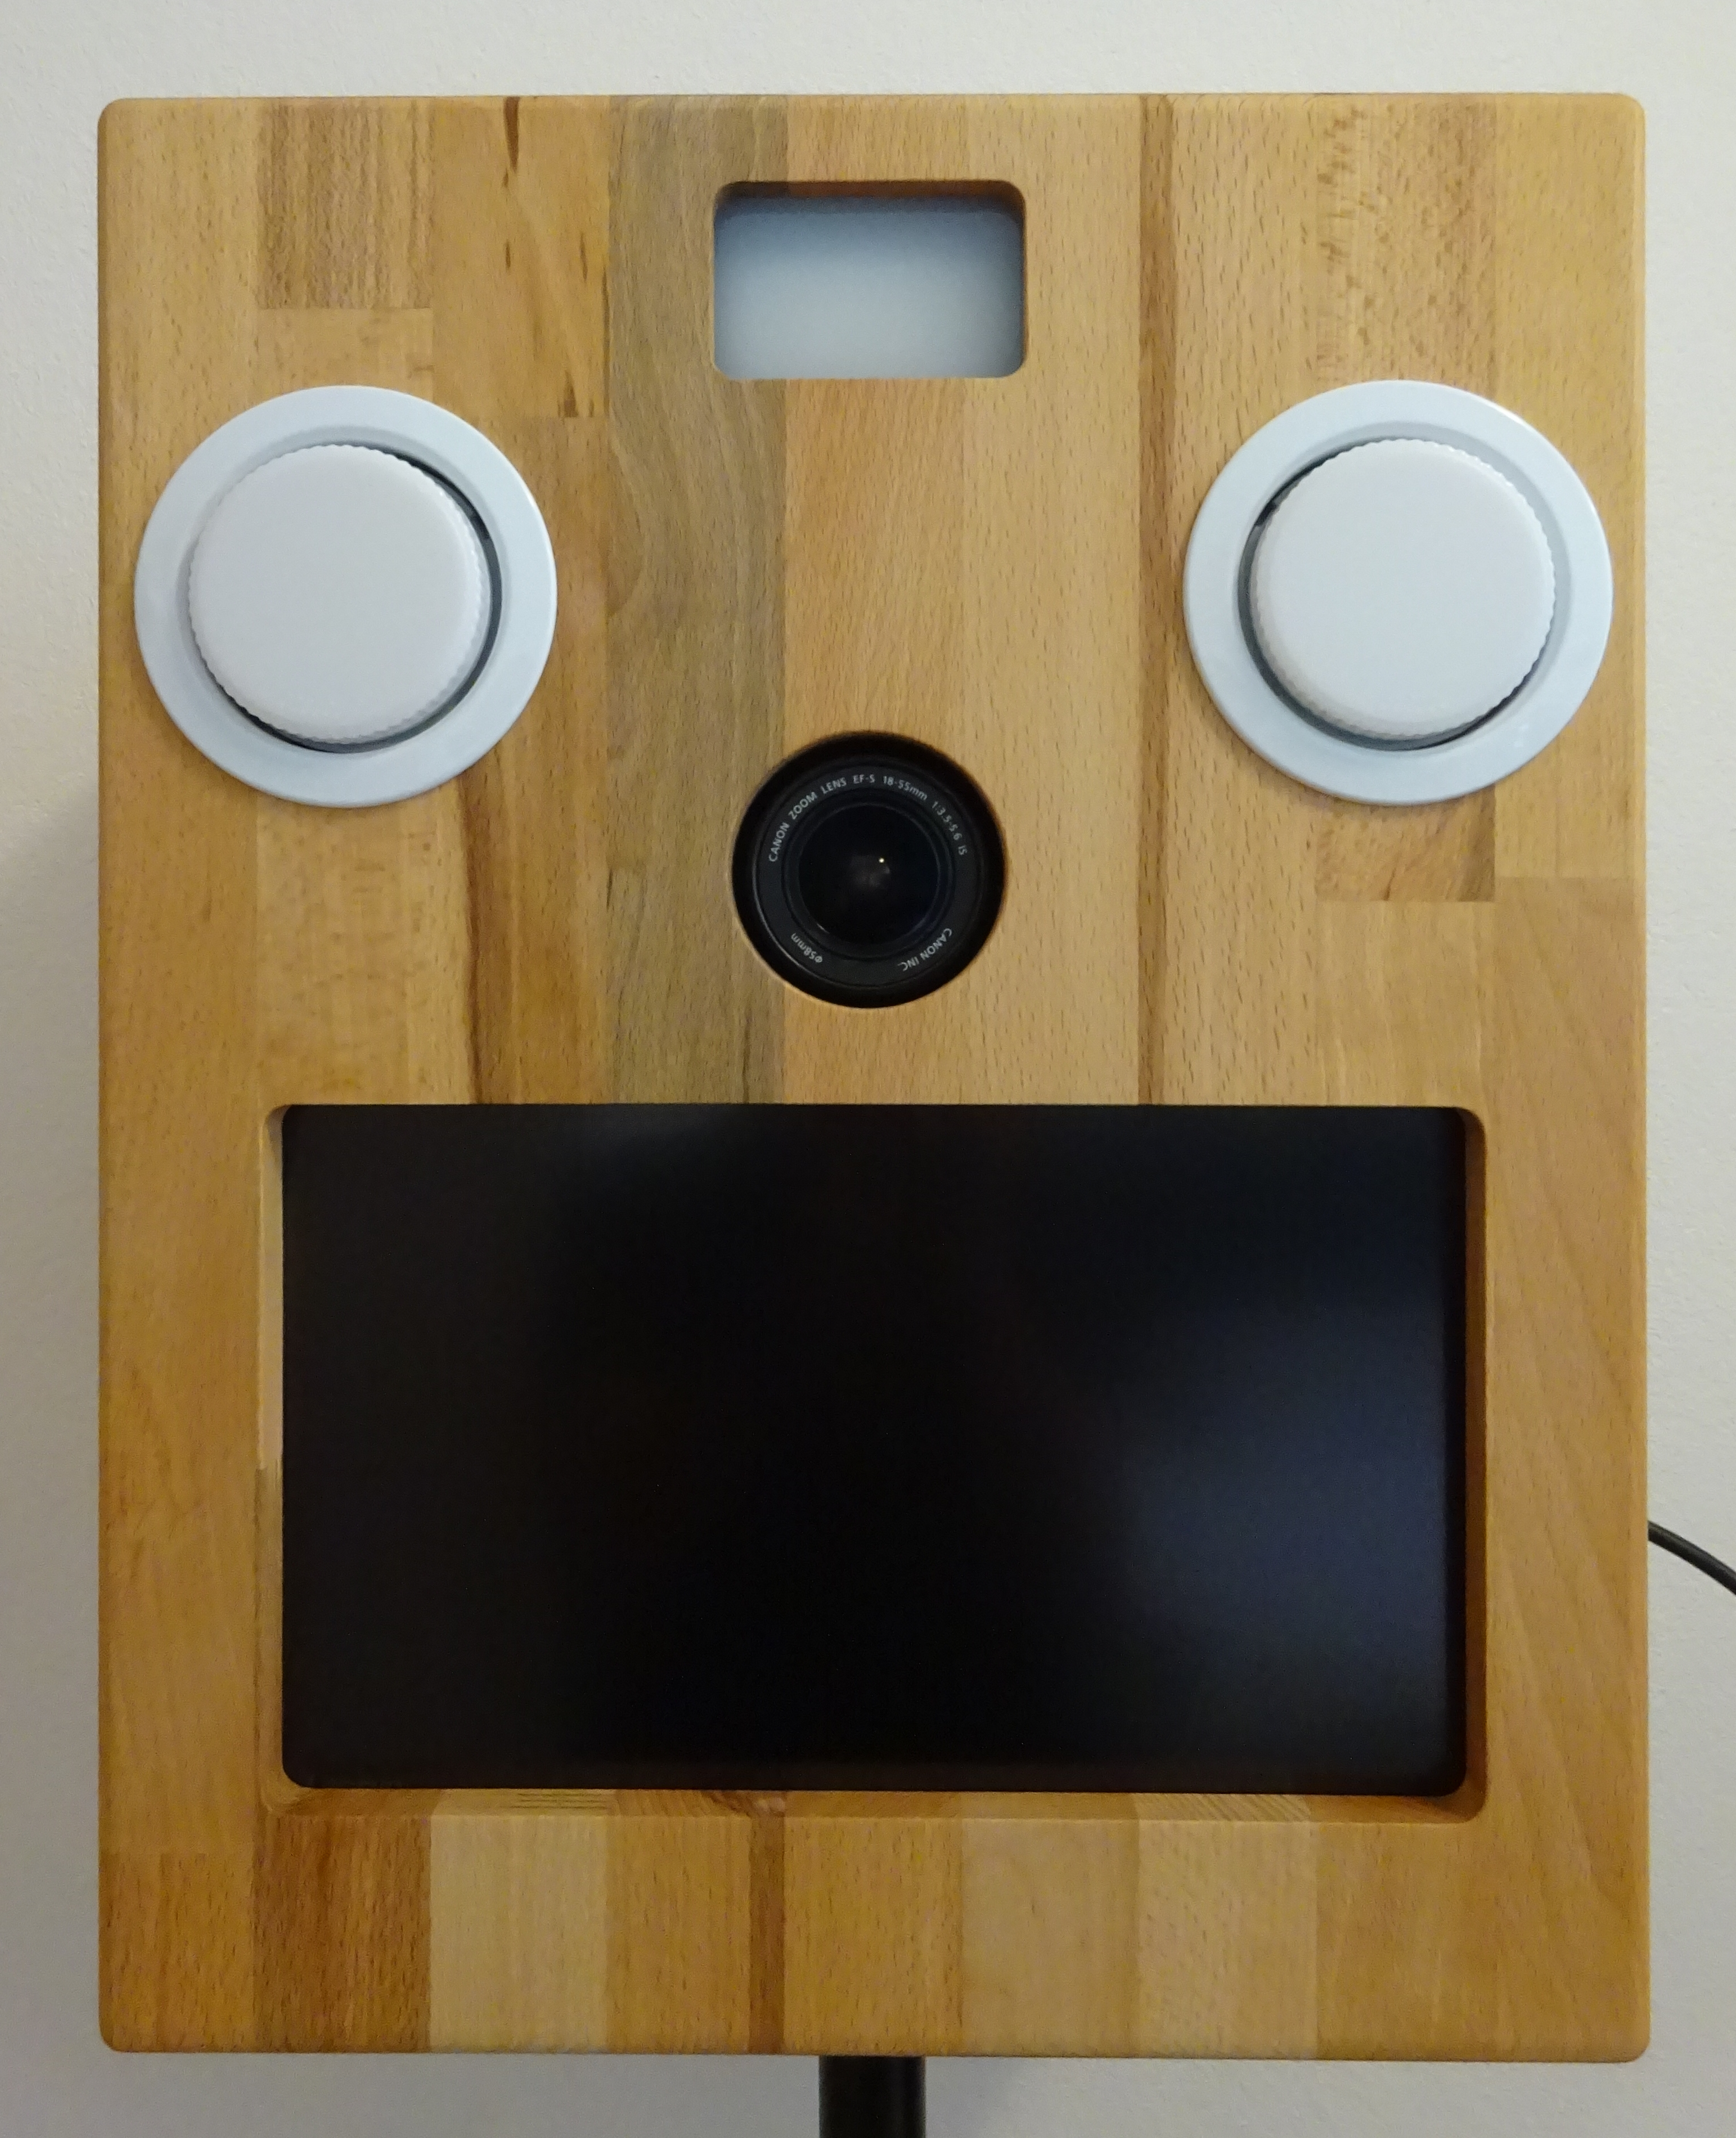
\includegraphics[width=0.75\textwidth]{images/mechanics/fotobox_fertig.JPG}
    \caption{Die fertige Box.}
    \label{fig:gewinde_schneiden}
\end{figure}